\documentclass[11pt]{article}
\usepackage[a4paper,margin=22mm,headheight=16pt]{geometry}
\usepackage{fontspec,xeCJK,xcolor,graphicx,enumitem,fancyhdr,titlesec}
\usepackage{hyperref}
\IfFontExistsTF{Times New Roman}{\setmainfont{Times New Roman}}{\setmainfont{TeX Gyre Termes}}
\IfFontExistsTF{FangSong}{\setCJKmainfont[AutoFakeBold=2]{FangSong}}{\IfFontExistsTF{仿宋}{\setCJKmainfont[AutoFakeBold=2]{仿宋}}{\IfFontExistsTF{FandolFang-Regular.otf}{\setCJKmainfont[AutoFakeBold=2]{FandolFang-Regular.otf}}{\setCJKmainfont{FandolSong-Regular.otf}}}}
\definecolor{ink}{HTML}{173747}\definecolor{accent}{HTML}{227E82}
\hypersetup{colorlinks=true,urlcolor=accent,linkcolor=accent}
\linespread{1.22}\setlength{\parindent}{0pt}\setlength{\parskip}{6pt}
\setlist[itemize]{leftmargin=1.4em,itemsep=3pt}
\titleformat{\section}{\large\bfseries\color{ink}}{}{0pt}{}
\titlespacing*{\section}{0pt}{14pt}{7pt}
\pagestyle{fancy}\fancyhf{}\lhead{\small OMNI LEARNING / 学习手册}\rhead{\small Source-grounded learning}\cfoot{\small\thepage}
\emergencystretch=2em\widowpenalty=10000\clubpenalty=10000
\newcommand{\Needspace}[1]{\par\ifdim\dimexpr\pagegoal-\pagetotal\relax<#1\relax\newpage\fi}
\begin{document}


{\LARGE\bfseries\color{ink} 建筑如何被阅读}\par

2026-10-08 | Day01/30 | 阅读 8 分钟 + 练习 3 分钟\par\vspace{6pt}

\Needspace{5\baselineskip}\section*{今日导航}

今天回答：面对一栋陌生建筑，除了说“漂亮”，还能看什么？目标是用空间、结构、用途和背景四个问题观察建筑，并区分平面、立面和剖面。课程以西方建筑史为主线，但不把它等同于全球建筑史。

\Needspace{5\baselineskip}\section*{从站在哪里开始}

你在一座教堂门前拍照，看到的是正面形象；走进去后，尺度、光线和路线可能完全改变体验。照片能提供信息，也会受镜头、光线和站位影响。建筑是可进入的空间，不只是立面上的图案。第一步可以问：人从哪里进入，往哪里走，什么地方允许停留？

\begin{center}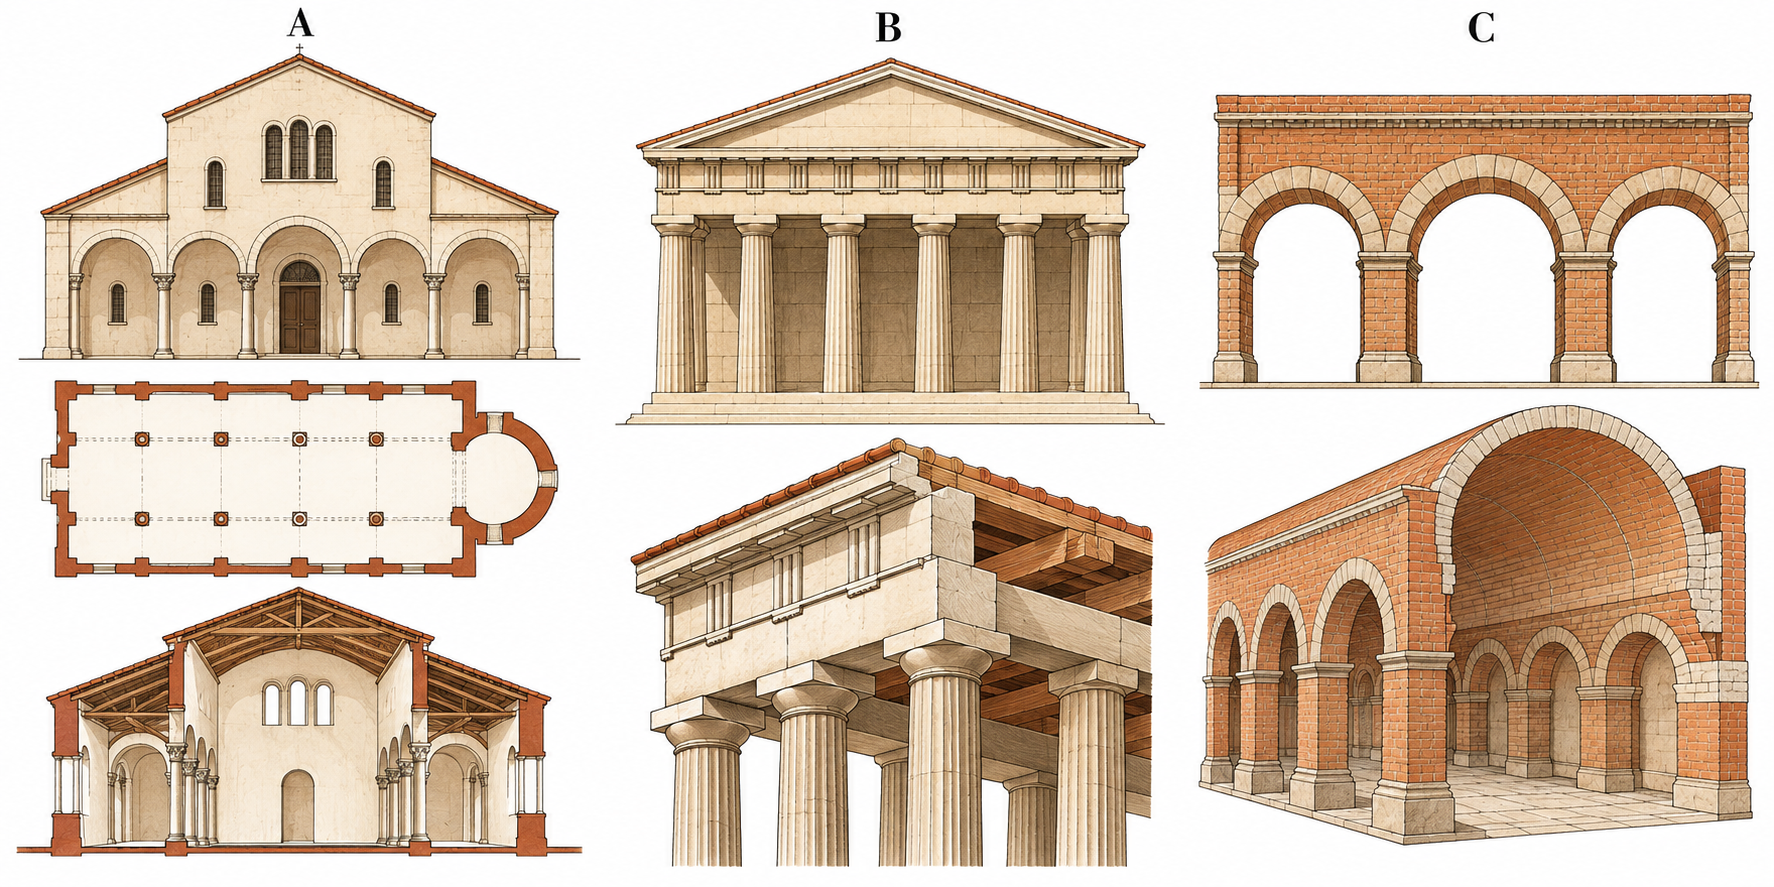
\includegraphics[width=\linewidth,height=0.26\textheight,keepaspectratio]{../assets/figure-9ba448966b26.png}\par

{\small 本课重点看 A 区。A 平面、立面与剖面提供不同信息；B 梁柱；C 拱券与桶形拱顶。图为类型示意，不是具体遗址测绘图。}\par

{\footnotesize AI生成教学示意，非实物照片、原始史料或官方架构。生成方式：内置文生图；提示词见仓库 docs/image-prompts.json。}\end{center}

\Needspace{5\baselineskip}\section*{三种图纸回答不同问题}

平面像在某个高度水平切开建筑后向下看，帮助辨认房间、柱墙与路线。立面表达从某一方向正看外部的形态。剖面则沿竖向切开，揭示层高、屋顶和空间之间的关系。图 A 用同一类建筑的概念示意帮助对照，但不是测绘资料，不能用它量尺寸。

再加四个观察问题：谁使用？怎样站得住？材料和施工怎样组织？在什么社会环境中形成？柱子可能承重，也可能参与装饰；大厅可能用于仪式，也可能用于公共活动。仅凭外形就断定用途或结构，需要额外证据。

\Needspace{5\baselineskip}\section*{用案例建立观察顺序}

罗马剧场材料把看台支撑、通道和观众安排联系起来，说明建筑形式与活动及社会组织有关。[S2] 今天不必记具体尺寸，只要理解同一空间可以同时解决工程问题和秩序问题。

旅行时建议先看现场说明确认年代与用途，再画一条主要行走路线，最后观察墙、柱、开口和屋顶怎样关联。像罗马历史中心这样的城市包含多个时期的叠加，不能因为地点在罗马就认定每座建筑都是古罗马式。[S4] 现存外观还可能包含修缮或改建，日期应对应具体部分。

\Needspace{5\baselineskip}\section*{三分钟练习与自查}

选择你熟悉的一座图书馆、商场或车站，写四句观察：进入路线、主要空间、可能的支撑方式、实际使用者。给不确定的判断加“需要核实”。

参考：“从广场进入大厅；大厅连接两条通道；屋顶似乎由边缘柱支撑，但需看剖面；使用者包括通勤者与商店顾客。”自查：是否把看见的事实和结构猜测分开？是否只描述了风格，没有考虑人在里面做什么？不会画专业图也不影响完成。

\Needspace{5\baselineskip}\section*{复盘与明日连接}

平面看组织，立面看外部，剖面看内部高度与联系；再把用途、结构、材料和背景连起来。明天从希腊柱式进入历史主线，理解一套形式规则如何组织整栋建筑，而不是只背几种柱头。

\Needspace{6\baselineskip}\section*{扩展学习 / Further reading}\small 以下为选读，不计入每日必做时间。\begin{enumerate}[leftmargin=1.6em]

\item [S1] \href{https://www.metmuseum.org/essays/architecture-in-ancient-greece}{Architecture in Ancient Greece} — 观察柱式如何连接立柱与建筑其他部分，而非只认柱头。\par The Metropolitan Museum of Art | 发布：2003-10-01 | 核验：2026-10-08

\item [S2] \href{https://www.metmuseum.org/essays/theater-and-amphitheater-in-the-roman-world}{Theater and Amphitheater in the Roman World} — 了解拱券、看台、通道与社会秩序之间的关系。\par The Metropolitan Museum of Art | 发布：2006-10-01 | 核验：2026-10-08

\item [S3] \href{https://whc.unesco.org/en/list/404/}{Acropolis, Athens} — 结合雅典卫城原址资料，区分单栋建筑与建筑群。\par UNESCO | 发布：未标注 | 核验：2026-10-08

\item [S4] \href{https://whc.unesco.org/en/list/91/}{Historic Centre of Rome} — 观察城市历史叠加；不要把罗马城市归为单一风格。\par UNESCO | 发布：未标注 | 核验：2026-10-08

\item [S5] \href{https://whc.unesco.org/en/list/81/}{Chartres Cathedral} — 为后续哥特建筑预习，关注结构、空间与彩色玻璃。\par UNESCO | 发布：未标注 | 核验：2026-10-08

\end{enumerate}

\end{document}